\documentclass[b4paper, landscape, dvipdfmx]{jsarticle}
%----- 必要なパッケージ -----
\usepackage{fancybox,ascmac,otf}
\usepackage{amssymb, amsthm}
\usepackage[leqno]{amsmath}
\usepackage{geometry}
\usepackage{multicol}
\usepackage{tcolorbox}
\usepackage{xcolor}
\usepackage{fancyhdr}
\usepackage{tikz}

% TikZライブラリ
\usetikzlibrary{
    positioning,
    arrows.meta,
    calc,
    shadows,
    shadows.blur,
    intersections,
    angles,
    quotes
}

% tcolorboxライブラリ
\tcbuselibrary{skins, breakable, theorems}

\usepackage{enumitem}
\setlist[enumerate,1]{label=(\arabic*)}
\setlist[itemize]{leftmargin=*}
\newcommand{\ds}{\displaystyle}

%----- レイアウト設定 -----
\geometry{
  left=15mm,
  right=15mm,
  top=20mm,
  bottom=15mm,
  headheight=25pt
}

%----- 数式環境の上下の余白調整 -----
\AtBeginDocument{
  \setlength{\abovedisplayskip}{5pt}
  \setlength{\belowdisplayskip}{5pt}
  \setlength{\abovedisplayshortskip}{0pt}
  \setlength{\belowdisplayshortskip}{3pt}
}

%===========================================================
%  デザイン設定
%===========================================================

%--- 色の定義 ---
\definecolor{printBlue}{RGB}{0, 50, 100}     % 濃紺
\definecolor{printRed}{RGB}{140, 20, 20}     % 濃エンジ
\definecolor{printTeal}{RGB}{0, 60, 60}      % 濃い青緑

%--- 共通スタイル定義 ---
\tcbset{
    chartbox/.style={
        enhanced,
        fonttitle=\sffamily\bfseries,
        boxrule=1pt,
        arc=2pt,
        top=1.0em,
        nobeforeafter,
        enlarge left by=-2mm,
        enlarge right by=-2mm,
        drop fuzzy shadow,
        colback=white,
        attach boxed title to top left={xshift=10pt, yshift*=-\tcboxedtitleheight/2},
        boxed title style={frame hidden, sharp corners, rounded corners=southeast, arc=3pt}
    }
}

%--- 各種ボックス環境定義 ---

% セクション・枠組み用 (any)
\newtcolorbox{any}[1]{
    enlarge left by=0mm, enlarge right by=0mm,
    enhanced, frame hidden, colback=white, title={#1},
    attach boxed title to top left={xshift=0mm, yshift=0mm},
    coltitle=white, fonttitle=\bfseries\sffamily,
    boxed title style={
        colback=black!80, frame hidden, arc=4pt, outer arc=4pt,
        sharp corners=south, boxrule=0pt,
        top=1mm, bottom=1mm, left=3mm, right=3mm
    },
    underlay boxed title={
        \draw[thick, black!80] (title.south west) -- (title.south west-|frame.east);
    },
    breakable, top=5mm, left=2mm, right=2mm, bottom=0mm,
    before skip=1em, after skip=1em,
    segmentation style={draw=black!40, dashed}
}

% 例題 (eg)
\newtcolorbox{eg}[1]{
    chartbox,
    colframe=printBlue,
    coltitle=white,
    title=\textbf{例題 #1},
    boxed title style={colback=printBlue},
    segmentation style={draw=printBlue, line width=0.5pt, dashed}
}

% 練習 (prac)
\newtcolorbox{prac}[1]{
    chartbox,
    colframe=printRed,
    coltitle=white,
    title=\textbf{練習 #1},
    boxed title style={colback=printRed}
}

% 定理 (thm)
\newtcolorbox{thm}[1]{
    chartbox,
    colframe=printTeal,
    coltitle=white,
    title=\textbf{#1},
    boxed title style={colback=printTeal}
}

% 解答欄 (answer)
\newtcolorbox{answer}[1][height fill]{
    enhanced,
    title={Memo / Answer},
    colframe=black!80,
    colback=white,
    coltitle=black!60,
    fonttitle=\sffamily\bfseries,
    attach boxed title to top left={xshift=5mm, yshift*=-\tcboxedtitleheight/2},
    boxed title style={frame hidden, colback=white},
    boxrule=1pt,
    arc=1pt,
    nobeforeafter,
    enlarge left by=-2mm, 
    enlarge right by=-2mm, 
    height fill,
    segmentation style={draw=black!20, solid},
    underlay={
        \begin{tcbclipinterior}
            \draw[step=5mm, black!5, ultra thin] (interior.south west) grid (interior.north east);
        \end{tcbclipinterior}
    }, 
    #1
}

%----- 段組の設定 -----
\setlength{\columnsep}{15mm}
\setlength{\columnseprule}{0.4pt}
\renewcommand{\columnseprulecolor}{\color{black!30}}

%----- ヘッダーの設定 -----
\pagestyle{fancy}
\fancyhf{}
\fancyhead[C]{%
    \begin{tikzpicture}[remember picture, overlay]
        \node[anchor=north west, fill=printBlue, minimum width=\paperwidth, minimum height=5pt] at (current page.north west) {};
    \end{tikzpicture}
}
\fancyhead[L]{\small \textcolor{black!90}{数学C $>$ 第1章--平面ベクトル $>$ 第5回 \textbf{成分による内積と垂直条件}}}
\fancyhead[R]{\small 年 \hspace{1cm} 組 \hspace{1cm} 番 \quad 氏名 \hspace{6cm}}
\renewcommand{\headrulewidth}{0pt}

\begin{document}

%=============================================================================
% 1枚目:成分による内積計算
%=============================================================================
\begin{multicols}{2}

%-----------------------------------------------------------------------------
% 左カラム:公式の導入
%-----------------------------------------------------------------------------
\begin{any}{1. 座標データから内積を計算する}
    前回, 内積は「長さと角度」で定義した ($\vec{a}\cdot\vec{b} = |\vec{a}||\vec{b}|\cos\theta$).
    しかし, 成分(座標)がわかっていれば, わざわざ角度を測らなくても内積を一発で計算できる.

    \begin{thm}{成分による内積の公式}
        $\vec{a} = (a_1, a_2), \vec{b} = (b_1, b_2)$ のとき,
        \[ \vec{a} \cdot \vec{b} = a_1 b_1 + a_2 b_2 \]
        つまり, \textbf{「$x$同士, $y$同士を掛けて足す」}だけでよい.
    \end{thm}

    \begin{tcolorbox}[colback=white, colframe=black!80, title={なぜこの式になる?(余弦定理との関係)}, fonttitle=\bfseries]
        \begin{minipage}{0.38\linewidth}
            \centering
            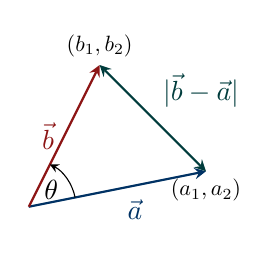
\begin{tikzpicture}[scale=0.9, >=stealth]
                \coordinate (O) at (0,0);
                \coordinate (A) at (2.5, 0.5);
                \coordinate (B) at (1, 2);
                
                \draw[->, thick, printBlue] (O) -- (A) node[midway, below right] {$\vec{a}$};
                \draw[->, thick, printRed] (O) -- (B) node[midway, left] {$\vec{b}$};
                \draw[<->, thick, printTeal] (A) -- (B) node[midway, above right] {$|\vec{b}-\vec{a}|$};
                
                \pic [draw, ->, "$\theta$", angle radius=0.6cm] {angle = A--O--B};
                
                \node[below, scale=0.8] at (A) {$(a_1,a_2)$};
                \node[above, scale=0.8] at (B) {$(b_1,b_2)$};
            \end{tikzpicture}
        \end{minipage}
        \hfill
        \begin{minipage}{0.60\linewidth}
            \small
            $\triangle OAB$ に余弦定理を適用する.
            \[ |\vec{b}-\vec{a}|^2 = |\vec{a}|^2 + |\vec{b}|^2 - 2|\vec{a}||\vec{b}|\cos\theta \]
            $|\vec{a}||\vec{b}|\cos\theta = \vec{a}\cdot\vec{b}$ より式変形すると:
            \begin{equation*}
                \vec{a}\cdot\vec{b} = \frac{1}{2} \left( |\vec{a}|^2 + |\vec{b}|^2 - |\vec{b}-\vec{a}|^2 \right)
            \end{equation*}
            ここで成分を代入する.
            \begin{itemize}
                \item $|\vec{a}|^2 = a_1^2 + a_2^2$
                \item $|\vec{b}|^2 = b_1^2 + b_2^2$
                \item $|\vec{b}-\vec{a}|^2 = (b_1-a_1)^2 + (b_2-a_2)^2$
            \end{itemize}
        \end{minipage}
        
        \vspace{0.5em}
        \hrule
        \vspace{0.5em}
        
        \textbf{代入して計算(項が綺麗に消える!):}
        \begin{align*}
             \vec{a}\cdot\vec{b} &= \frac{1}{2} \{ (a_1^2+a_2^2) + (b_1^2+b_2^2) - (b_1-a_1)^2 - (b_2-a_2)^2 \} \\
             &= \frac{1}{2} \{ \not{a_1^2}+\not{a_2^2} + \not{b_1^2}+\not{b_2^2} - (\not{b_1^2}-2a_1b_1+\not{a_1^2}) - (\not{b_2^2}-2a_2b_2+\not{a_2^2}) \} \\
             &= \frac{1}{2} ( 2a_1b_1 + 2a_2b_2 ) = \boldsymbol{a_1b_1 + a_2b_2}
        \end{align*}
    \end{tcolorbox}

    \begin{eg}{1 (成分計算となす角)}
        $\vec{a}=(1, \sqrt{3}), \vec{b}=(\sqrt{3}, 1)$ のとき,
        \begin{enumerate}
            \item 内積 $\vec{a} \cdot \vec{b}$ を求めよ.
            \item $\vec{a}, \vec{b}$ のなす角 $\theta$ を求めよ.
        \end{enumerate}
        \tcblower
        \vspace{8cm}
    \end{eg}
\end{any}

%-----------------------------------------------------------------------------
% 右カラム:垂直条件
%-----------------------------------------------------------------------------
\columnbreak

\begin{any}{2. 垂直条件 (Perpendicular Condition)}
    内積の定義より, ベクトルが垂直ならば $\cos 90^\circ = 0$ なので内積は0になる.
    これを成分で表すと強力な武器になる.

    \begin{thm}{垂直条件}
        $\vec{a} \neq \vec{0}, \vec{b} \neq \vec{0}$ のとき,
        \[ \vec{a} \perp \vec{b} \iff \vec{a} \cdot \vec{b} = 0 \iff a_1 b_1 + a_2 b_2 = 0 \]
        「垂直」というワードを見たら, 条件反射で\textbf{「内積=0」}の式を作る.
    \end{thm}
    
    \textbf{応用(垂直なベクトルの作り方):} \\
    $(a, b)$ に垂直なベクトルのひとつは $(b, -a)$ である.
    \[ a \times b + b \times (-a) = ab - ab = 0 \]
    
    \begin{eg}{2 (垂直なベクトル)}
        $\vec{a} = (3, 1)$ に垂直で, 大きさが $\sqrt{10}$ であるベクトル $\vec{x}$ をすべて求めよ.
        \tcblower
        \textbf{方針:}
        未知数が2つ ($x$成分, $y$成分) なので式が2つ必要.
        \begin{itemize}
            \item 垂直条件: $\vec{a} \cdot \vec{x} = 0$
            \item 大きさ条件: $|\vec{x}| = \sqrt{10}$
        \end{itemize}
        これらを連立する.
        \vspace{6cm}
    \end{eg}
\end{any}

\end{multicols}

%=============================================================================
% 2枚目:確認テスト(問題)
%=============================================================================
\newpage
\fancyhead[L]{\small \textcolor{black!90}{数学C $>$ 第1章--平面ベクトル $>$ 第5回--\textbf{確認テスト}}}
\begin{multicols}{2}

\begin{any}{確認テスト (A: 基本)}
    \begin{prac}{A1 (成分計算)}
        次のベクトルの内積 $\vec{a} \cdot \vec{b}$ を求めよ.
        \begin{enumerate}
            \item $\vec{a} = (2, -5), \quad \vec{b} = (3, 2)$
            \item $\vec{a} = (1, 0), \quad \vec{b} = (0, 1)$
            \item $\vec{a} = (-1, -1), \quad \vec{b} = (1, -1)$
        \end{enumerate}
    \end{prac}
    \begin{answer}[height=5cm]
    \end{answer}

    \begin{prac}{A2 (なす角)}
        $\vec{a} = (2, 1), \vec{b} = (-3, 1)$ のなす角 $\theta$ を求めよ.
        \[ \cos\theta = \frac{\vec{a} \cdot \vec{b}}{|\vec{a}| |\vec{b}|} \]
        を利用する.
    \end{prac}
    \begin{answer}[height=5cm]
    \end{answer}
\end{any}

\columnbreak

\begin{any}{確認テスト (B: 標準)}
    \begin{prac}{B1 (垂直条件)}
        $\vec{a} = (x-1, 3), \vec{b} = (2, x)$ が垂直になるような実数 $x$ の値を求めよ.
    \end{prac}
    \begin{answer}[height=6cm]
    \end{answer}

    \begin{prac}{B2 (垂直な単位ベクトル)}
        $\vec{a} = (4, 3)$ に垂直な\textbf{単位ベクトル} $\vec{e}$ を求めよ.
    \end{prac}
    \begin{answer}[height=6cm]
    \end{answer}
\end{any}

\end{multicols}

%=============================================================================
% 3枚目:確認テスト(解答)
%=============================================================================
\newpage
\fancyhead[L]{\small \textcolor{black!90}{数学C $>$ 第1章--平面ベクトル $>$ 第5回 \textbf{【解答解説】}}}

\begin{multicols}{2}

\begin{any}{解答 (A: 基本)}
    \begin{prac}{A1 (成分計算)}
        (1) $2 \times 3 + (-5) \times 2 = 6 - 10 = \boldsymbol{-4}$ \\
        (2) $1 \times 0 + 0 \times 1 = \boldsymbol{0}$ (直交している) \\
        (3) $(-1)\times 1 + (-1)\times (-1) = -1 + 1 = \boldsymbol{0}$
    \end{prac}

    \begin{answer}[height=8cm]
    \color{printRed}
    \textbf{A2 解答:} \\
    まずは内積とそれぞれの大きさを計算する.
    \begin{itemize}
        \item 内積: $\vec{a} \cdot \vec{b} = 2(-3) + 1(1) = -6 + 1 = -5$
        \item 大きさ: $|\vec{a}| = \sqrt{2^2+1^2} = \sqrt{5}$ \\
        \phantom{大きさ: } $|\vec{b}| = \sqrt{(-3)^2+1^2} = \sqrt{10}$
    \end{itemize}
    よって,
    \begin{align*}
        \cos\theta &= \frac{-5}{\sqrt{5} \sqrt{10}} = \frac{-5}{\sqrt{50}} = \frac{-5}{5\sqrt{2}} \\
        &= -\frac{1}{\sqrt{2}}
    \end{align*}
    $0^\circ \leqq \theta \leqq 180^\circ$ より, $\boldsymbol{\theta = 135^\circ}$
    \end{answer}
\end{any}

\columnbreak

\begin{any}{解答 (B: 標準)}
    \begin{answer}[height=6cm]
    \color{printRed}
    \textbf{B1 解答:} \\
    垂直条件より, 内積が 0 になればよい.
    \begin{align*}
        (x-1) \cdot 2 + 3 \cdot x &= 0 \\
        2x - 2 + 3x &= 0 \\
        5x &= 2 \\
        \therefore \quad x &= \frac{2}{5}
    \end{align*}
    \end{answer}

    \begin{answer}[height fill]
    \color{printRed}
    \textbf{B2 解答:} \\
    求める単位ベクトルを $\vec{e}=(x, y)$ とおく.
    \begin{itemize}
        \item 垂直条件: $4x + 3y = 0 \implies x = -\frac{3}{4}y$ \dots(1)
        \item 単位ベクトル(大きさ1): $x^2 + y^2 = 1$ \dots(2)
    \end{itemize}
    (1)を(2)に代入:
    $(-\frac{3}{4}y)^2 + y^2 = 1 \implies \frac{9}{16}y^2 + y^2 = 1$ \\
    $\frac{25}{16}y^2 = 1 \implies y^2 = \frac{16}{25} \implies y = \pm \frac{4}{5}$.
    
    $y = \frac{4}{5}$ のとき $x = -\frac{3}{5}$. \quad $y = -\frac{4}{5}$ のとき $x = \frac{3}{5}$.
    
    よって, $\boldsymbol{\vec{e} = (-\frac{3}{5}, \frac{4}{5}), \ (\frac{3}{5}, -\frac{4}{5})}$
    
    \vspace{1em}
    \textbf{別解 (テクニック):} \\
    $(4, 3)$ に垂直なベクトルの1つは $(3, -4)$.
    この大きさは $\sqrt{3^2+(-4)^2} = 5$.
    これを大きさ1に縮めればよいので, $\pm \frac{1}{5}(3, -4)$.
    \end{answer}
\end{any}

\end{multicols}
\end{document}